\documentclass{biophys_letter}
\usepackage{dcolumn,color,helvet,times}
%\usepackage{ulem}
\usepackage{soul}
\usepackage[usenames,dvipsnames]{xcolor}
\usepackage{amsmath,lastpage,bm,textcomp}%mathtime
\usepackage{multicol}
\usepackage{cite} % my own added packages
\jno{kxl014} %journal number
\gridframe{N} %option for grid around the text "Y" or "N"
\cropmark{N} %option for cropmark around the text "Y" or "N"

\doi{doi: XX.XXXX/biophysj.XXX.XXXXXX}% DOI number in the copyright line

% macros (from macros.tex)
%% OPTIONAL MACRO DEFINITIONS
\newcommand{\argmax}{\operatornamewithlimits{argmax}}
\newcommand{\argmin}{\operatornamewithlimits{argmin}}
\newcommand{\ifrac}[2]{#1 \:/\: #2}

%% MODEL TERMS
\newcommand{\bias}{\beta}
\newcommand{\err}{\epsilon}

%% ADDRESS LINE MACROS
\def\authdag{{\fontsize{5.65}{6}$^{\mbox{\textdagger}}$}}
\def\authddag{{\fontsize{5.65}{6}$^{\mbox{\textdaggerdbl}}$}}
\def\authS{{\fontsize{5.65}{6}$^{\mbox{\textsection}}$}}
\def\authpar{{\fontsize{5.65}{6}$^{\mbox{\textparagraph}}$}}
\def\addrdag{{\fontsize{7.07}{8}$^{\mbox{\textdagger}}$}}
\def\addrddag{{\fontsize{7.07}{8}$^{\mbox{\textdaggerdbl}}$}}
\def\addrS{{\fontsize{7.07}{8}$^{\mbox{\textsection}}$}}
\def\addrpar{{\fontsize{7.07}{8}$^{\mbox{\textparagraph}}$}}

%% COMMENTS
\newcommand{\jwm}[1]{\textcolor{Magenta}{#1}}
%\newcommand{\jwm}[1]{#1}
\newcommand{\kje}[1]{\textcolor{BurntOrange}{#1}}
%\newcommand{\kje}[1]{#1}
\newcommand{\chw}[1]{\textcolor{OliveGreen}{#1}}
%\newcommand{\chw}[1]{#1}
\newcommand{\jkr}[1]{\textcolor{RawSienna}{#1}}
%\newcommand{\jkr}[1]{#1}
\newcommand{\kls}[1]{\textcolor{MidnightBlue}{#1}}
%\newcommand{\kls}[1]{#1}
\newcommand{\com}[1]{\{\emph{#1}\}}
%\newcommand{\com}[1]{}

% use parens instead of brackets in cite command
\makeatletter
\renewcommand\@cite[1]{(#1)}
\makeatother

\title{Statistical Inference for Nanopore Sequencing with a Biased Random Walk Model}

\author{Kevin J. Emmett,{\authdag *} Jacob K. Rosenstein,{\authpar} Jan-Willem van de Meent,{\authddag} Ken L. Shepard,{\addrS} and Chris H. Wiggins{\authddag}}
\address{{\addrdag}Department of Physics and {\addrddag}Department of Applied Physics and Applied Math and {\addrS}Department of Electrical Engineering, Columbia University, New York, New York; and {\addrpar}School of Engineering, Brown University, Providence, Rhode Island}

% document
\begin{document}

\setcounter{page}{1} %first page number

\markboth{Biophysical Journal: Biophysical Letters}{Biophysical Journal: Biophysical Letters} %for running head
\pagestyle{headings}

\maketitle

%Abstract environment needs 3 arguments. They are
%1. The abstract
%2. Received date
%3. Address, email

\begin{abstract}
{Nanopore sequencing promises long read-lengths and single-molecule resolution, but the stochastic motion of the DNA molecule inside the pore is a current barrier to high accuracy reads.
We develop a method of statistical inference that explicitly accounts for this error and demonstrate that high accuracy (\textgreater 99\%) sequence inference is feasible even under highly diffusive motion by using a hidden Markov model to jointly analyze multiple stochastic reads.
Using this model, we place bounds on achievable inference accuracy under a range of experimental parameters.}
{Received for publication 31 July 2013 and in final form 31 July 2013.}
{*Correspondence: kje@phys.columbia.edu.}
\end{abstract}

\begin{multicols}{2}

Rapid advances in DNA sequencing technologies have led to an explosion in available nucleotide sequence data, greatly enhancing our understanding of the genomic basis of many biological processes.
However, the short length of the raw reads means high coverage is required for reliable sequence assembly.
Nanopore sequencing has emerged as a candidate to supercede current generation sequencing and allow for theoretically unlimited read length \cite{Branton:2008}.
A number of strategies have been proposed, with the common basis of detecting individual nucleotides as they pass through a nanometer-scale aperture in a thin membrane separating two electrolytes \cite{Winters-Hilt:2004}.
To date, a significant obstacle of nanopore approaches has been overcoming the fast stochastic motion of the individual molecules as they are driven through the pore \cite{Venkatesan:2011, Lu:2011}.
Ideally, passage of DNA through the pore would be unidirectional and each base would have a well-resolved signal.
Recent methods have demonstrated an ability to controllably `ratchet' DNA molecules through a nanopore one base at a time, although motion of the molecule can still occur in both forward and backward directions within a single read \cite{Olasagasti:2010, Cherf:2012}.
Unidirectional motion remains difficult to reliably achieve, leading to a source of error in the read sequence recognized, but not previously addressed, by existing models.

%\kje{For accurate nanopore sequencing, diffusion should be minimized, as backwards motion will result in erroneous base-calls.}
In this letter, we analyze the effect of diffusive motion on achievable read accuracy and propose a statistical method to \kje{account} this error.
%To do so, we simulate noisy data where the true sequence is unknown, and develop a statistical technique to estimate the most likely DNA sequence associated with the simulated read signal.
Our method uses hidden Markov models (HMMs), which have recently been used to study multi-base resolution in a nanopore sequencer \cite{Timp:2012}, but have not yet been applied to the problem of diffusive motion inside the pore.
We show that combining multiple reads from a given input DNA sequence allows accurate estimates of the sequence, both in the presence of highly diffusive molecular motion and high base-call error rates.

\kje{
Polymer translocation through a nanopore is modeled as one-dimensional diffusion with driving force $F$ and a sampling interval equal to unit-nucleotide steps, $\tau=a/\left\langle\bar{v}\right\rangle$.
Here $a$ is the nucleotide width, and $\left\langle\bar{v}\right\rangle=F/\gamma$ is the average translocation velocity, where the drag coefficient $\gamma=1.27 \mathrm{\mu g/s}$ is calibrated using \cite{Lu:2011}.
The forward bias can be modeled with a dimensionless parameter $\beta$, given by %\cite{Berg:1993}
\begin{equation}
\label{eq:bias_term}
\bias = \frac{1}{\exp(-Fa/k_{B}T) + 1}.
\end{equation}
In this formulation, a transition, $\delta$, can occur forward or backward a given number of bases with probability $P(\tau,\delta)$.
Assuming no DNA-pore interaction, we can write this as a Gaussian diffusion kernel with transition probabilities
\begin{equation}
\label{eq:gaussian_kernel}
P(\tau,\delta) = \int\limits_{-3a/2+\delta a}^{-a/2+\delta a}\frac{1}{\sqrt{4\pi D\tau}}\exp\left(-\frac{x^2}{4D\tau}\right)\,dx
\end{equation}
with diffusion coefficient $D=a^2/2\tau$.
}
% Polymer translocation through a nanopore is modeled as one-dimensional diffusion with driving force $F$ and a dimensionless step size $a/\tau=1$ \cite{Lubensky:1999}.
%We model motion through the nanopore as one-dimensional diffusion with driving force $F$ and unit base step size $a$, and assume no DNA-pore interaction.
% Assuming no DNA-pore interaction, we can write this as a random walk with fixed forward bias \cite{Berg:1993}
% \begin{equation}
% %  \bias = \frac{1}{2} + \frac{Fa}{4k_{B}T},
%   \bias = \frac{1}{\exp(-Fa/k_{B}T) + 1}
% \end{equation}
% with diffusion coefficient $D=a^2/2\tau$ and drift velocity $v = a(2\bias-1)/\tau$.}


Given an input DNA sequence of length $L$, we generate a single output read by stepping through the sequence with a bias $\bias$, at each step making a base-call with error probability $\err$, which is independent of error introduced due to backward motion.
Finally, we assume an appropriate method of making a base-call from the raw signal, which has been computationally studied in \cite{ODonnell:2013}.
From this simple physical model, we generate a set of $N$ simulated reads $X_n$, each having a unique length $T_{n}$.
$N$ is a notion of sequence coverage in terms of identical molecules sequenced, which could result from either amplification or resequencing of the initial molecule.
A schematic representation of a nanopore sequencing device is shown in Fig.~\ref{fig:fig1}\emph{~A}.
\kje{
In Fig.~\ref{fig:fig1}\emph{~B} we plot the relationship between forward bias, driving force, and the sampling frequency required for single base resolution.
In Fig.~\ref{fig:fig1}\emph{~C} we plot $P(\tau,\delta)$ at several different forward biases.
In Fig.~\ref{fig:fig1}\emph{~D} the distribution of read lengths at these forward biases is shown.
}
% In Fig.~\ref{fig:fig1}\emph{~B} a series of random walks at several different forward biases is shown, along with the read length distribution, equivalent to the first passage distribution.
% With an average translocation velocity $v$, the expected length of a read is
% \begin{equation}
%   \label{eq:expected-T}
%   \left\langle T  \right\rangle = \frac{L}{v} = \frac{1}{2\bias-1} L.
% \end{equation}

\end{multicols}
\twocolumn

Given the set of $N$ read sequences, the statistical task is to infer the sequence most likely to have generated the observed data.
An experiment similar to this model was demonstrated on very short sequences with tunneling current data in \cite{Ohshiro:2012}.
Here we extend the approach to the longer sequences expected from a nanopore device.

% figure 1. cartoon and random walk model
\begin{figure}
  \centering
  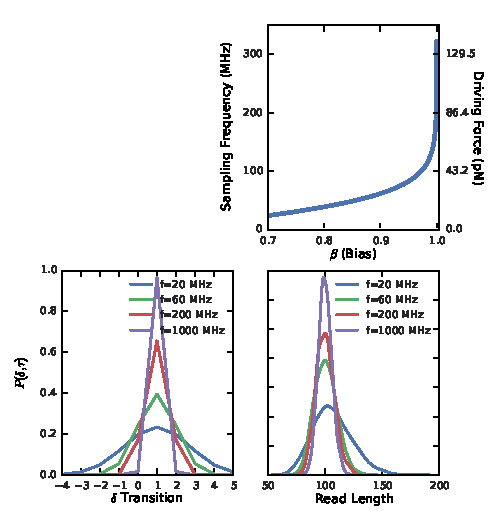
\includegraphics[width=3.25in]{fig/fig1_new.pdf}
  \caption{Random walk model of nanopore sequencing. (A) Schematic representation of an idealized nanopore sequencing device. (B) Relationship between forward bias, driving force and sampling frequency. Quoted sampling frequency is the minimum required for single base resolution. (C) Transition probabilities and (D) read length distributions for different sampling frequencies (sequence length $L=100$).}
  \label{fig:fig1}
\end{figure}

In our HMM formulation, each output read is modeled as a discrete set of observed states, $\mathbf{x}=\{x_{1}\dots x_{T}\}$, $x_i \in (A,C,G,T)$, a vector of observed bases, and a discrete set of hidden states, $\mathbf{z}=\{z_{1} \dots z_{T}\}$, $z_i \in (1 \dots L)$, the unknown position along the sequence.
An HMM is described by three model parameters, the initial state distribution $\pi=p(\mathbf{z}_{1})$, the hidden state transition matrix $A=p(\mathbf{z}_{t}\:|\:\mathbf{z}_{t-1})$, and an emission distribution $S=p(\mathbf{x}_{n}\:|\:\mathbf{z}_{n})$.
$\pi$ and $A$ are fixed by the experimental conditions.
\kje{The elements of $A$ are obtained by numerically integrating Eq.~\ref{eq:gaussian_kernel} over possible transitions, $\delta$.}
The inference problem in this model is to estimate the emission distribution, $S$, which acts as an implicit representation of our sequence,
\begin{equation}
  S_{dl} = (1-\err)p(\mathbf{x}_n = d\:|\:\mathbf{z}_{n} = l) + \err/4
\end{equation}
In practice, $S$ is a $4 \times L$ matrix with a multinomial distribution over the possible nucleotides at each position (see Fig.~\ref{fig:inference_output}).
\kje{We use the expectation-maximization algorithm to maximize the likelihood, $p(X \:|\: \theta)$, with respect to the model parameters \cite{Baum:1970}.}
% We maximize the likelihood, $p(X \:|\: \theta)$, with respect to the model parameters using an implementation of the expectation-maximization algorithm \cite{Baum:1970}.
The joint probability of data and states can be written as a product over the independent output reads, $p(\mathbf{X},\mathbf{Z}\:|\:\theta)=\prod_{n}p(\mathbf{X}_n,\mathbf{Z}_n\:|\:\theta)$, from which follows that we can perform expectation updates on each read individually before averaging results in the maximization step (see Supporting Material for full model derivation).
The resulting shared parameter estimation scheme incorporates all reads while allowing an efficient, parallel calculation.

After a convergence criterion on the likelihood is satisfied (${\Delta}LL<10^{-5}$), we recover an estimated emission distribution $S$, which can be converted to an estimate for the DNA sequence by taking $\mathrm{\max_{d}} {S_{dl}}$.
The final inference accuracy is measured as the Levenstein distance between the input sequence and inferred sequence, normalized by $L$.
The algorithm has complexity $O(NLT)$, where $T$ is $O(L)$ in the limit of $\bias=1$.
An example of the output of this algorithm showing the relationship between the true sequence and the inferred sequence distribution is shown in Fig.~\ref{fig:inference_output}\emph{~A}.
% Additionally, the column-wise entropy of the sequence inference, defined as $H_{l}=-\sum_{d}S_{dl}\log{S_{dl}}$, is plotted above.
%\kje{As shown, large regions of the sequence are correctly inferred, with errors in the form of spurious insertion and deletion artifacts.}
%\kje{Inference errors in are generally associated with increases in the inference entropy around the error position $l$, where the algorithm cannot distinguish between backwards motion and repeat base patterns.}
% \kje{\st{
% Inference errors, which can be identified with insertion and deletion artifacts where the algorithm cannot distinguish between backwards motion and repeat base patterns, are associated with increases in $H_{l}$.
% This suggests a possible approach that further analysis might employ to systematically identify and remove inference errors due to bidirectional motion.
% }}

% figure 2: inference output
\begin{figure}
  \centering
  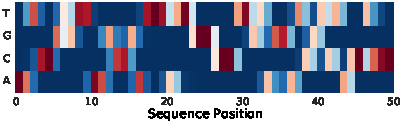
\includegraphics[width=3.25in]{fig/fig2_new.pdf}
  \caption{The output of the statistical model and its relationship to the true sequence. (A) The output sequence inference distribution, $S$. (B) Taking $\argmax$ of each columns yields the sequence inference.}
  \label{fig:inference_output}
\end{figure}

We examined the performance of the algorithm over a range of parameter values in order to identify a minimal experimental configuration capable of sequence inference at a given accuracy.
First, we consider how to select realistic values for our parameters.
$\bias=0.5$ corresponds to completely symmetric diffusion and is unlikely to reach the end of the sequence without first exiting from the {\it cis} side of the nanopore (these reads are discarded in the data generation).
$\bias=1.0$ corresponds to nondiffusive motion and is a trivial case in this model.
Lu et al. report an experimental bias term of $Fa/4k_{B}T=0.2$ ($\bias=0.69$), for which they show single-pass accurate sequence recovery is impossible \cite{Lu:2011}.
We take this as a starting point for investigation, exploring the range $\bias=0.7$ to $\bias=1.0$.
An appropriate base-call error rate will be device specific and is presently unknown, so we examine the range $\err=0.0$ to $\err=0.5$.
The number of reads, $N$, is potentially unlimited, and we examine until convergence.

% figure 3: parameter sweeps
\begin{figure}
  \centering
  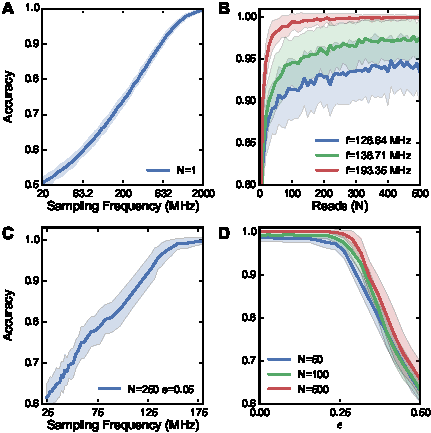
\includegraphics[width=3.25in]{fig/fig3_new.pdf}
  \caption{Parameter Sweeps. Inference accuracy (measured as 1 - Levenshtein distance/length) is plotted as a function of experimental parameters. (A) Baseline performance for a single read, $N=1$. (B) Parameter sweep across number of reads, $N$. (C) Asymptotic performance (large $N$) performance vs forward bias $\bias$. (D) error rate $\err$ vs $N$. Accuracy is independent of error rate.}
  \label{fig:parameter_sweeps}
\end{figure}

A sweep across the parameter space is shown in Fig.~\ref{fig:parameter_sweeps}.
For \emph{N}=1, the average inference accuracy goes roughly as \kje{{\raise.17ex\hbox{$\scriptstyle\sim$}}$\log{(f)}$} until saturating, a baseline measure of performance (Fig. \ref{fig:parameter_sweeps}\emph{~A}).
In Fig.~\ref{fig:parameter_sweeps}\emph{~B} we plot the relationship between bias and the number of reads.
As expected, the strongest determinant of inference accuracy is the number of reads, \emph{N}.
This is expected because each read contributes an independent observation of the input DNA sequence.
We observe an inference error rate that falls rapidly with increasing \emph{N}, even at highly diffusive motion.
Generally, the achievable accuracy converges at a fixed $\bias$ even with the addition of more reads.
This asymptotic performance is plotted in Fig.~\ref{fig:parameter_sweeps}\emph{~C}.
A threshold accuracy of 99\% is achievable for $\bias=0.8$ ($Fa/4k_{B}T=0.35$); an accuracy exceeding 99.9\% is achievable with $\bias>0.88$ ($Fa/4k_{B}T>0.50$).
These results suggest accurate sequencing is possible at driving forces much lower than previously thought.
Finally, inference accuracy is \kje{robust to base-call error rates up to 30\%}, provided each nucleotide in the sequence is visited sufficient times (Fig.~\ref{fig:parameter_sweeps}\emph{~D}).

\kje{Unidirectional} motion of the DNA sequence inside the nanopore has been assumed a necessary prerequisite for accurate nanopore sequencing.
% Precise control over the motion of the DNA sequence inside the nanopore has been assumed a necessary prerequisite for accurate nanopore sequencing.
We have demonstrated that high accuracy inference is possible, even in the presence of diffusive motion, with the integration of data under an appropriate statistical model.
The strength of the method lies in the way in which multiple reads of the input sequence are independently modeled and then iteratively combined to yield a joint estimate of the true sequence.
Under this model, reasonably accurate sequence inference is achievable even within the experimental constraints of today's nanopore devices ($\bias\approx 0.7$).
More complicated translocation dynamics can be incorporated in model through modification to the state transition matrix.
Designers of nanopore sequencers may find that there is a tradeoff between sequencing speed and maintaining unidirectional molecular motion.
In this scenario, techniques such as the random walk model may allow increased throughput without a loss of accuracy.

\section*{SUPPORTING MATERIAL}

The full inference model is available at BPJ Online. Source code used to perform the analysis will be available at \\http://stochseq.github.io.

\section*{ACKNOWLEDGEMENTS}

The authors gratefully acknowledge helpful discussions with David Blei, Frank Wood, and David Pfau.

KJE and CHW were supported by NIH grant U54-CA121852 (National Center for Multiscale Analysis of Genomic and Cellular Networks). JWM was supported through the NWO Rubicon Fellowship 680-50-1016. KLS was supported by NIH grant R01-HG006879.

\begin{thebibliography}{99}

\bibitem{Branton:2008}
  Branton, D., Deamer, D. W., Marziali, A., Bayley, H., Benner, S. A., Butler, T., et al.
  2008.
  The potential and challenges of nanopore sequencing.
  {\it Nat. Biotechnol.}
  26:1146---1153.

\bibitem{Winters-Hilt:2004}
  Winters-Hilt, S., and M. Akeson.
  2004.
  Nanopore cheminformatics.
  {\it DNA and Cell Biology}
  23:675--683

\bibitem{Venkatesan:2011}
  Venkatesan, B. M., and R. Bashir.
  2011.
  Nanopore sensors for nucleic acid analysis.
  {\it Nat. Nanotechnol.}
  6:615---624.

\bibitem{Lu:2011}
  Lu, B., F. Albertorio, D. P. Hoogerheide, and J. A. Golovchenko.
  2011.
  Origins and consequences of velocity fluctuations during DNA passage through a nanopore.
  {\it Biophys. J.}
  101:70---79.

\bibitem{Luan:2011}
  Luan, B., H. Peng, S. Polonsky, S. Rossnagel, G. Stolovitzky, and G. Martyna.
  2010.
  Base-by-base ratcheting of single stranded DNA through a solid-state nanopore.
  {\it Phys. Rev. Lett.}
  104:238103.

\bibitem{Olasagasti:2010}
  Olasagasti, F., K. R. Lieberman, S. Benner, G. M. Cherf, J. M. Dahl, D. W. Deamer, and M. Akeson.
  2010.
  Replication of individual DNA molecules under electronic control using a protein nanopore.
  {\it Nat. Nanotechnol.}
  5:798--806.

\bibitem{Cherf:2012}
  Cherf, G. M., K. R. Lieberman, H. Rashid, C. E. Lam, K. Karplus, and M. Akeson.
  2012.
  Automated forward and reverse ratcheting of DNA in a nanopore at 5{\AA} precision.
  {\it Nat. Biotechnol.}
  30:344--348.

\bibitem{Lubensky:1999}
  Lubensky, D. K., and D. R. Nelson.
  1999.
  Driven Polymer Translocation Through a Narrow Pore.
  {\it Biophys. J.}
  77:1824--1838

\bibitem{Timp:2012}
  Timp, W., J. Comer, and A. Aksimentiev.
  2012.
  DNA base-calling from a nanopore using a Viterbi algorithm.
  {\it Biophys. J.}
  102:L37---L39

% \bibitem{Berg:1993}
%   Berg, H. C.
%   1993.
%   Random Walks in Biology.
%   Princeton University Press.
%   Princeton, New Jersey.

\bibitem{ODonnell:2013}
  O'Donnell, C. R., H. Wang, and W. B. Dunbar.
  2013.
  Error analysis of idealized nanopore sequencing.
  {\it Electrophoresis}
  In press.

\bibitem{Ohshiro:2012}
  Ohshiro, T., K. Matsubara, M. Tsutsui, M. Furuhashi, M. Taniguchi, and T. Kawai.
  2012.
  Single-Molecule electrical random resequencing of DNA and RNA.
  {\it Scientific Reports}
  2:1--7.

\bibitem{Rabiner:1989}
  Rabiner, L. R.
  1989.
  A tutorial on hidden Markov models and selected applications in speech recognition.
  {\it P. IEEE.}
  77:257---286.

\bibitem{Baum:1970}
  Baum, L. E., T. Petrie, G. Soules, and N. Weiss.
  1970.
  A maximization technique occurring in the statistical analysis of probabilistic functions of Markov chains.
  {\it Ann. Math. Stat.}
  41:164---171.

\bibitem{Dempster:1977}
  Dempster, A. P., N. M. Laird, and D. B. Rubin.
  1977.
  Maximum likelihood from incomplete data via the EM algorithm.
  {\it J. Roy. Stat. Soc. B. Met.}
  39:1---38.

\end{thebibliography}

\end{document}
